
%================================
\subsection{Comparación Pthreads vs OpenMP}
\label{sec:Comparación Pthreads vs OpenMP}

Haciendo las comparaciones etre los resultados obtenidos en el Caso de Estudio 1 donde se usó Pthreads y los resultados obtenidos en el Caso de Estudio 2 donde se usó OpenMP, se puede observar que ambos enfoques presentan mejoras significativas en el tiempo de ejecución a medida que se incrementa el número de hilos. Sin embargo, OpenMP tiende a mostrar un mejor rendimiento en comparación con Pthreads, especialmente cuando se utilizan más hilos. Esto se debe a que OpenMP está diseñado para facilitar la paralelización y optimización automática, mientras que Pthreads requiere una gestión manual de los hilos y la sincronización, lo que puede introducir sobrecarga adicional. En general, OpenMP es una opción más eficiente y fácil de usar para la multiplicación de matrices en entornos de programación paralela. En esta comparación se usaron los mejores resultados obtenidos para cada enfoque, tanto para Pthreads como para OpenMP con optimización por compilador como sin optimización por compilador.


\subsubsection{Resultados sin optimización por compilador}
\label{sec:Resultados sin optimización por compilador}

\begin{table}[H]
   \centering
   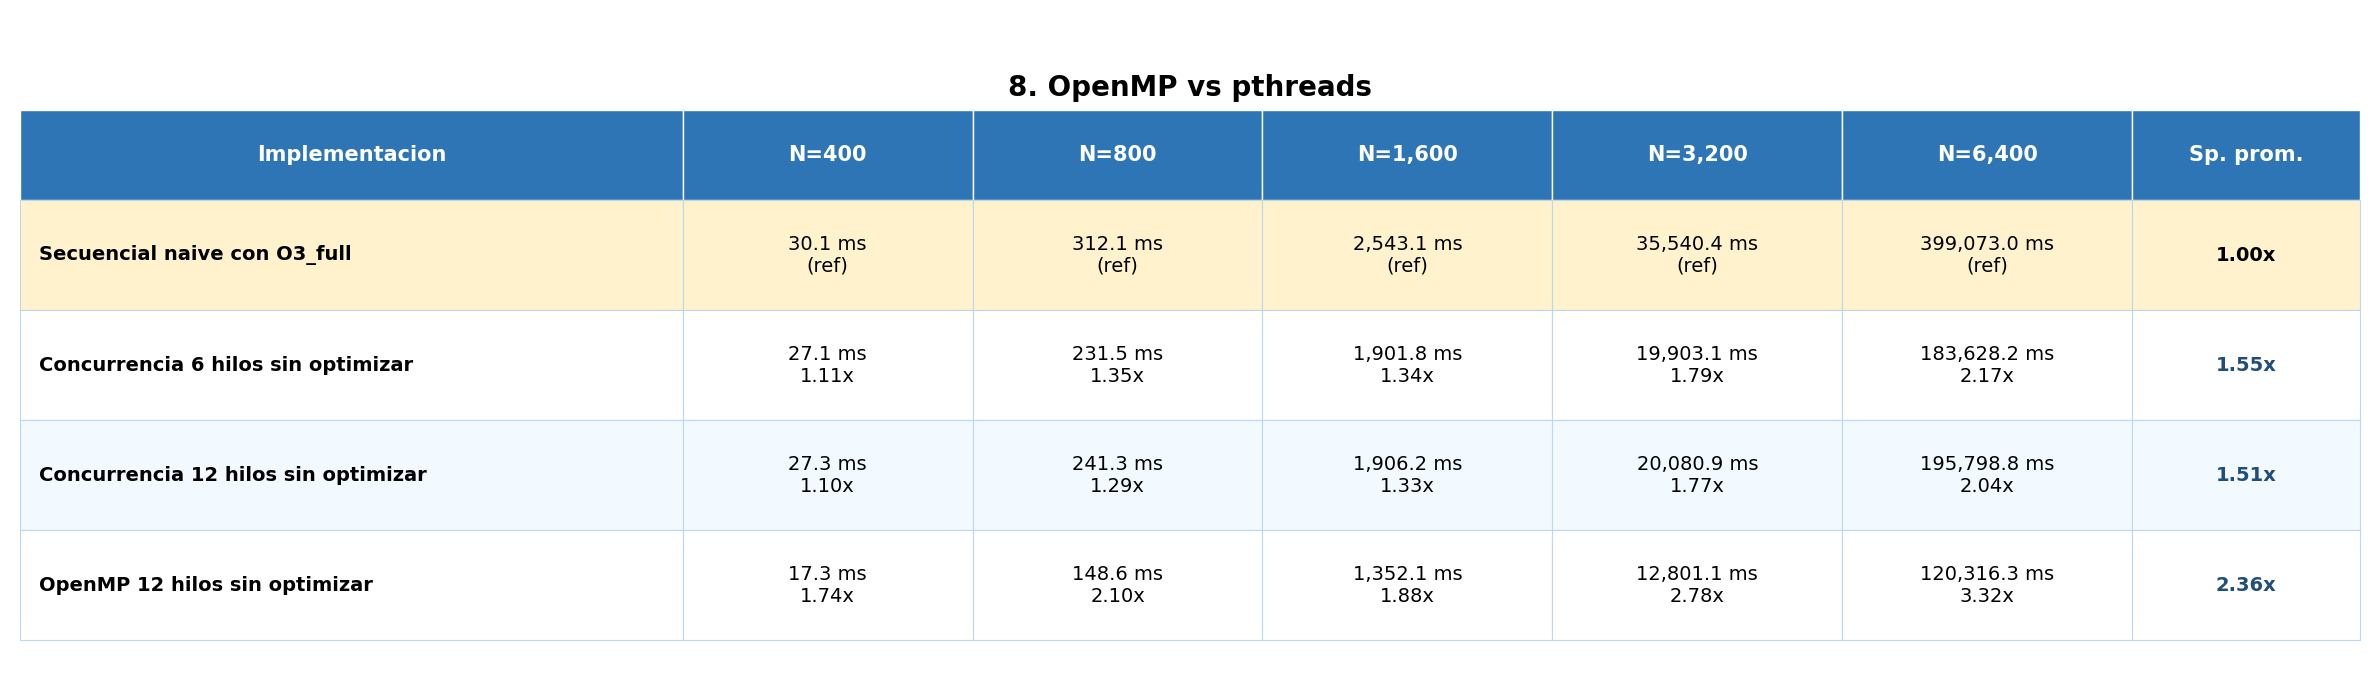
\includegraphics[width=1\textwidth]{images/omp/tables/table_omp_vs_threads.png}
   \caption{Comparación de tiempo de ejecución entre OpenMP y Pthreads para la multiplicación de matrices}
   \label{tab:comparison_omp_pthreads}
\end{table}

\begin{figure}[H]
   \centering
   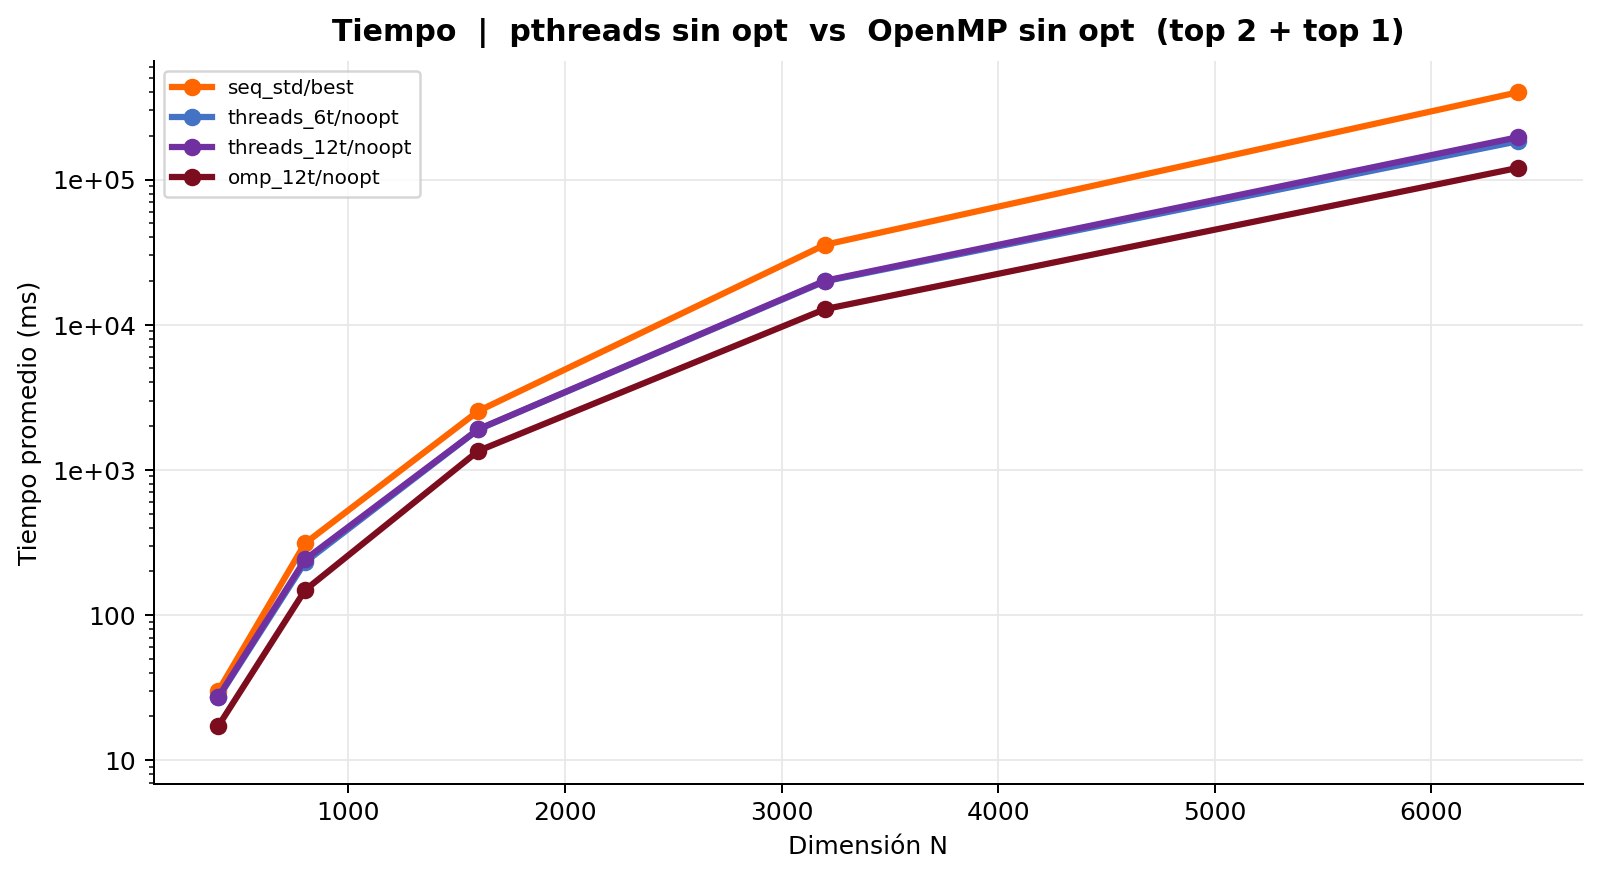
\includegraphics[width=1\textwidth]{images/omp/charts/time_pthreads_vs_omp.png}
   \caption{Gráfica de comparación de tiempo de ejecución entre OpenMP y Pthreads para la multiplicación de matrices}
\end{figure}

\begin{figure}[H]
   \centering
   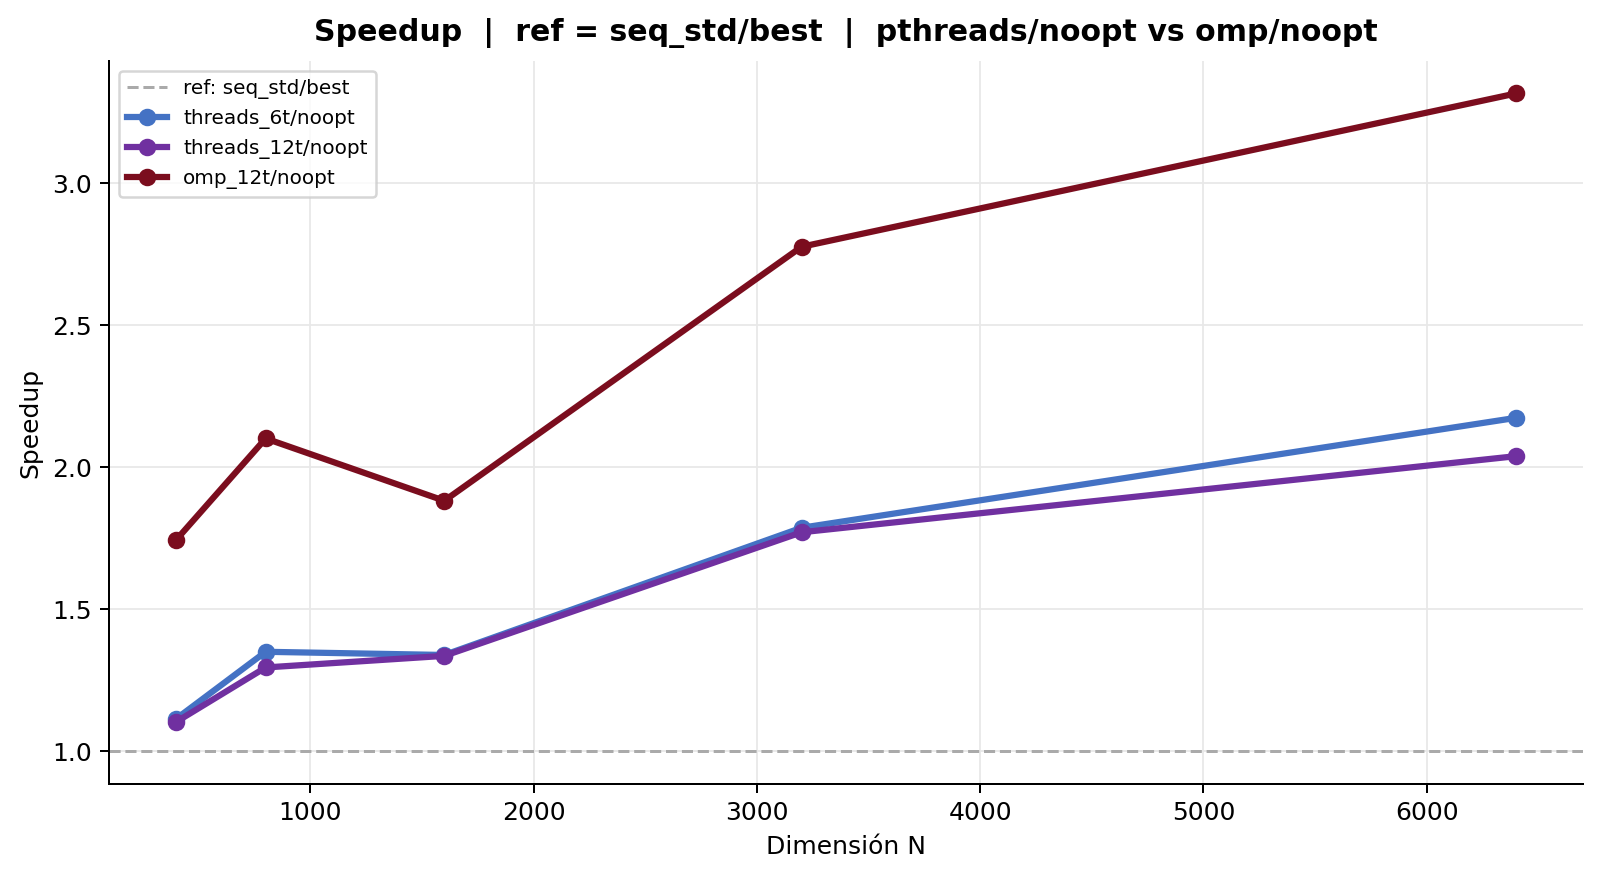
\includegraphics[width=1\textwidth]{images/omp/charts/speedup_pthreads_vs_omp.png}
   \caption{Gráfica de comparación de Speedup entre OpenMP y Pthreads para la multiplicación de matrices}
\end{figure}

\subsubsection{Resultados con optimización por compilador}

\begin{table}[H]
   \centering
   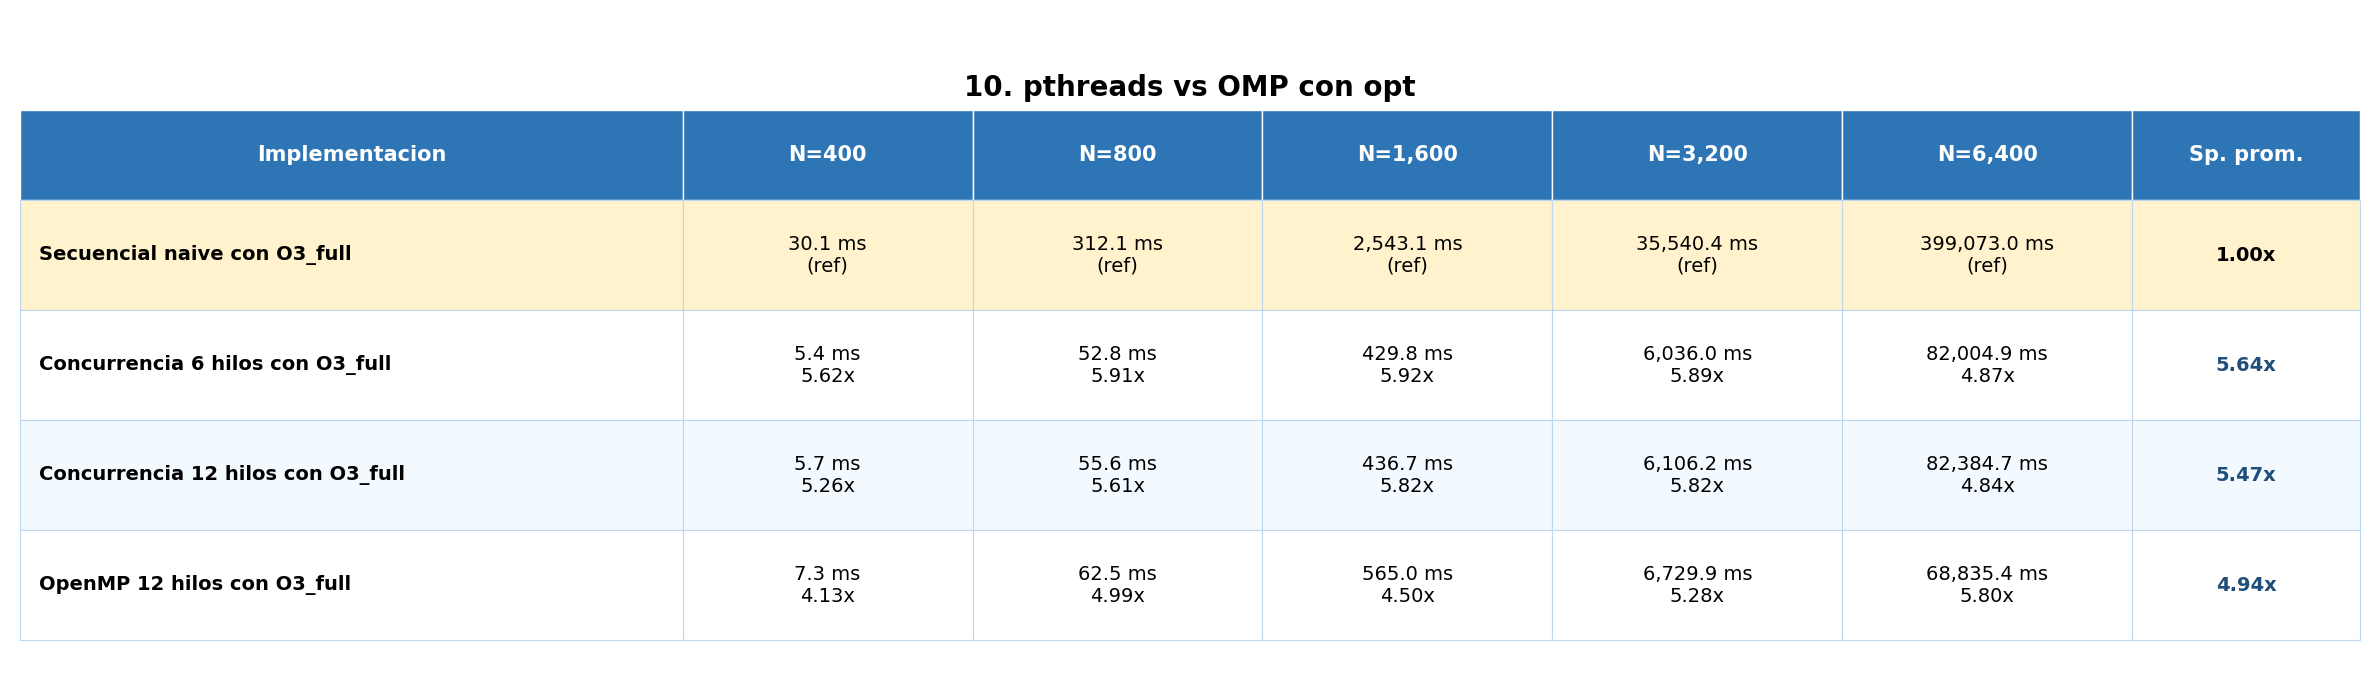
\includegraphics[width=1\textwidth]{images/omp/tables/table_pt_vs_omp_best.png}
   \caption{Comparación de tiempo de ejecución entre OpenMP y Pthreads para la multiplicación de matrices}
   \label{tab:comparison_omp_pthreads_opt}
\end{table}

\begin{figure}[H]
   \centering
   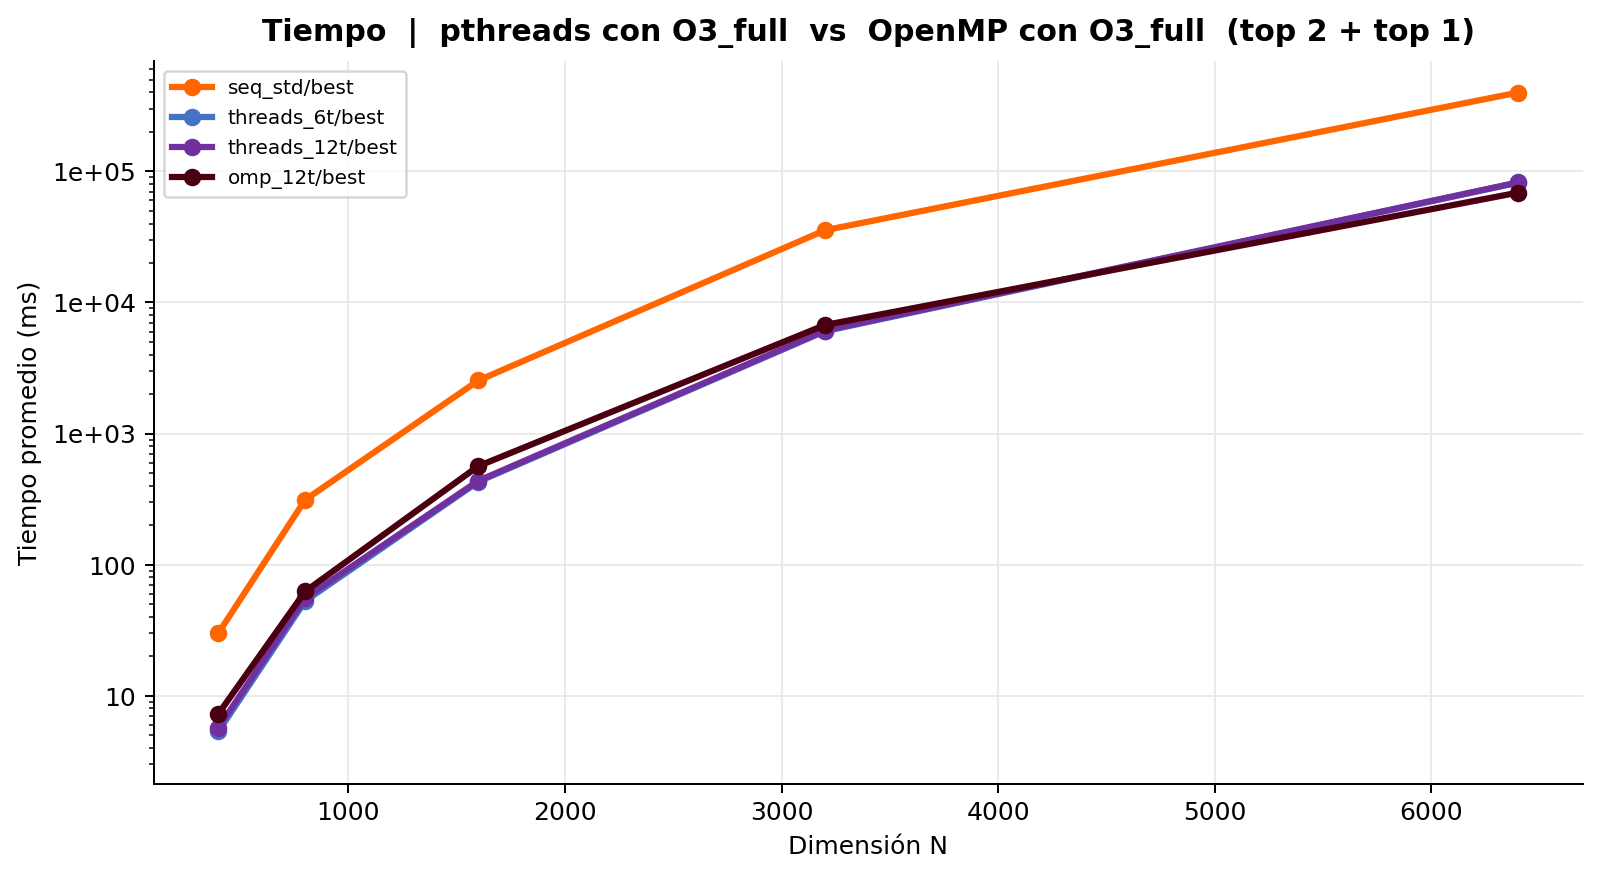
\includegraphics[width=1\textwidth]{images/omp/charts/time_pthreads_vs_omp_opt.png}
   \caption{Gráfica de comparación de tiempo de ejecución entre OpenMP y Pthreads para la multiplicación de matrices}
\end{figure}

\begin{figure}[H]
   \centering
   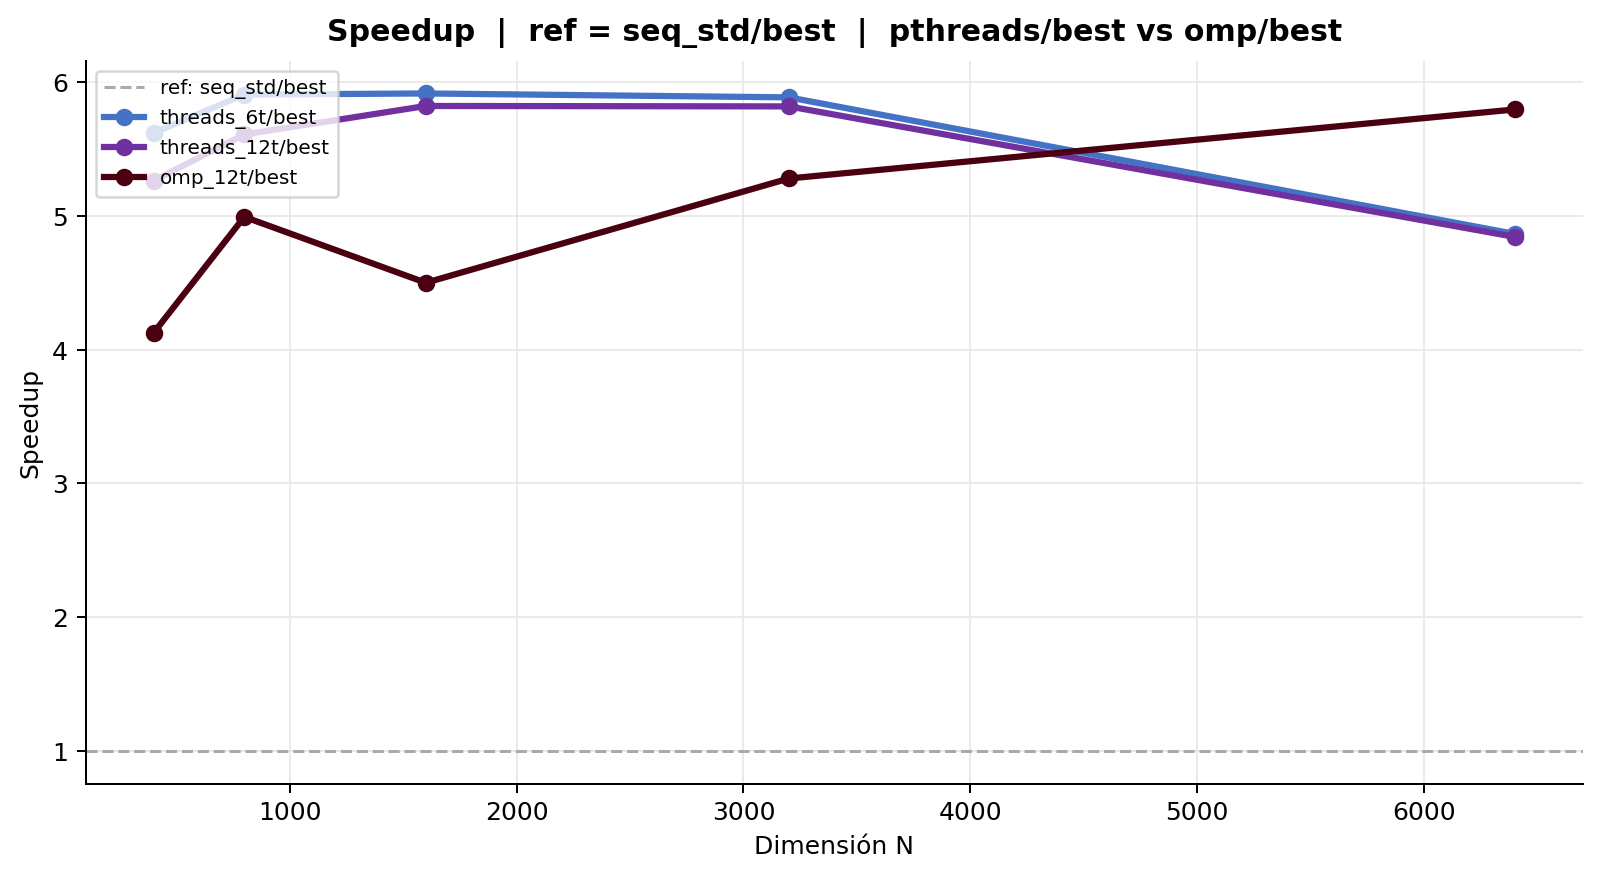
\includegraphics[width=1\textwidth]{images/omp/charts/speedup_pthreads_vs_omp_opt.png}
   \caption{Gráfica de comparación de Speedup entre OpenMP y Pthreads para la multiplicación de matrices}
\end{figure}

Aquí se observa algo interesante, la version con Pthreads optmizada por compilador tiene un mejor que la version con OpenMP optimizada por compilador en los tamaños más pequeños, pero a medida que el tamaño de las matrices aumenta, OpenMP con optimización por compilador supera a Pthreads con optimización por compilador, mostrando un mejor rendimiento y speedup. Esto puede deberse a que OpenMP está diseñado para aprovechar mejor los recursos del sistema y reducir el overhead asociado con la paralelización, mientras que Pthreads puede tener limitaciones en la gestión de hilos y sincronización a medida que el tamaño del problema aumenta.